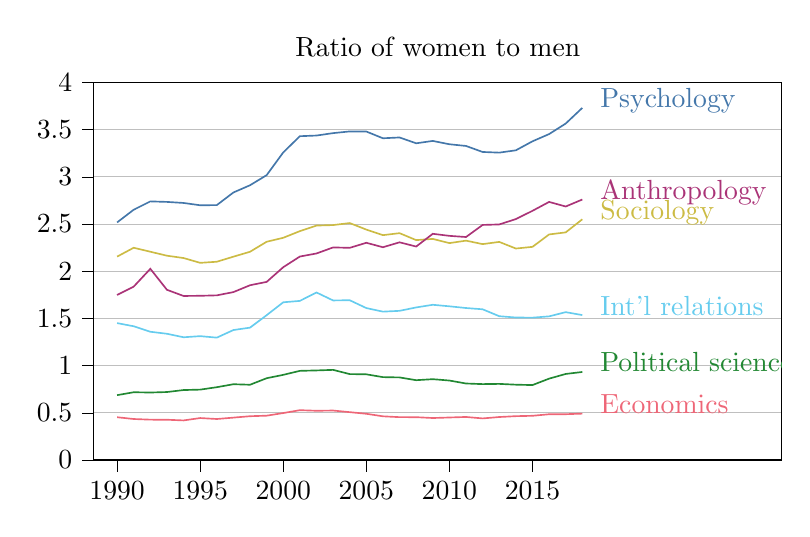
\begin{tikzpicture}
% This file was created with tikzplotlib v0.9.17.
\definecolor{color0}{rgb}{0.266666666666667,0.466666666666667,0.666666666666667}
\definecolor{color1}{rgb}{0.933333333333333,0.4,0.466666666666667}
\definecolor{color2}{rgb}{0.133333333333333,0.533333333333333,0.2}
\definecolor{color3}{rgb}{0.8,0.733333333333333,0.266666666666667}
\definecolor{color4}{rgb}{0.4,0.8,0.933333333333333}
\definecolor{color5}{rgb}{0.666666666666667,0.2,0.466666666666667}

\begin{axis}[
height=6.376357092455836cm,
tick align=outside,
tick pos=left,
title={Ratio of women to men},
width=10.317162499999998cm,
x grid style={white!69.0196078431373!black},
xmin=1988.6, xmax=2030,
xtick style={color=black},
xtick={1990,1995,2000,2005,2010,2015},
xticklabels={
  \(\displaystyle 1990\),
  \(\displaystyle 1995\),
  \(\displaystyle 2000\),
  \(\displaystyle 2005\),
  \(\displaystyle 2010\),
  \(\displaystyle 2015\)
},
ymajorgrids,
ymin=0, ymax=4,
ytick style={color=black},
ytick={0,0.5,1,1.5,2,2.5,3,3.5,4},
yticklabels={
  \(\displaystyle 0\),
  \(\displaystyle 0.5\),
  \(\displaystyle 1\),
  \(\displaystyle 1.5\),
  \(\displaystyle 2\),
  \(\displaystyle 2.5\),
  \(\displaystyle 3\),
  \(\displaystyle 3.5\),
  \(\displaystyle 4\)
}
]
\addplot [semithick, color0]
table {%
1990 2.5175244808197
1991 2.6520824432373
1992 2.74022936820984
1993 2.7347571849823
1994 2.72362613677979
1995 2.69927859306335
1996 2.70083546638489
1997 2.83463954925537
1998 2.9113347530365
1999 3.01813840866089
2000 3.2591769695282
2001 3.43097972869873
2002 3.43798732757568
2003 3.46344590187073
2004 3.48158049583435
2005 3.48040509223938
2006 3.40909743309021
2007 3.41750979423523
2008 3.35590291023254
2009 3.38099837303162
2010 3.34576916694641
2011 3.32759737968445
2012 3.26378393173218
2013 3.256920337677
2014 3.28145527839661
2015 3.37682676315308
2016 3.45335793495178
2017 3.56493353843689
2018 3.73112607002258
};
\addplot [semithick, color1]
table {%
1990 0.453454494476318
1991 0.434512615203857
1992 0.427694320678711
1993 0.426904916763306
1994 0.419453144073486
1995 0.444806575775146
1996 0.434596300125122
1998 0.464142203330994
1999 0.469876527786255
2000 0.497728705406189
2001 0.528073787689209
2002 0.521972298622131
2003 0.524367094039917
2005 0.490026116371155
2006 0.463130831718445
2007 0.454207539558411
2008 0.453919529914856
2009 0.445038676261902
2011 0.456213235855103
2012 0.440835237503052
2013 0.455652236938477
2014 0.464651584625244
2015 0.468673825263977
2016 0.484934091567993
2017 0.485498905181885
2018 0.491626977920532
};
\addplot [semithick, color2]
table {%
1990 0.687340497970581
1991 0.718239784240723
1992 0.715183019638062
1993 0.720339775085449
1994 0.741496920585632
1995 0.745949029922485
1996 0.771579146385193
1997 0.803107261657715
1998 0.797616720199585
1999 0.866689205169678
2000 0.902498960494995
2001 0.944846391677856
2002 0.949172735214233
2003 0.955212831497192
2004 0.910499453544617
2005 0.908062338829041
2006 0.878212213516235
2007 0.87516725063324
2008 0.845878720283508
2009 0.856622457504272
2010 0.84217095375061
2011 0.810709953308105
2012 0.804367065429688
2013 0.806700944900513
2014 0.798325777053833
2015 0.794228196144104
2016 0.862247109413147
2017 0.911926984786987
2018 0.932909369468689
};
\addplot [semithick, color3]
table {%
1990 2.15509796142578
1991 2.24903225898743
1993 2.16480875015259
1994 2.14018177986145
1995 2.08914875984192
1996 2.10084676742554
1997 2.15451312065125
1998 2.20654559135437
1999 2.31257438659668
2000 2.35462379455566
2001 2.42530727386475
2002 2.48414301872253
2003 2.48934626579285
2004 2.51065826416016
2005 2.44160652160645
2006 2.38261532783508
2007 2.40375828742981
2008 2.33004307746887
2009 2.34272146224976
2010 2.29821467399597
2011 2.32439589500427
2012 2.28757739067078
2013 2.31100392341614
2014 2.24083662033081
2015 2.25853753089905
2016 2.39009857177734
2017 2.41193509101868
2018 2.55055665969849
};
\addplot [semithick, color4]
table {%
1990 1.45081532001495
1991 1.41702950000763
1992 1.35909819602966
1993 1.33774352073669
1994 1.30062794685364
1995 1.31255269050598
1996 1.29666662216187
1997 1.37724554538727
1998 1.40262174606323
1999 1.53457581996918
2000 1.67128205299377
2001 1.6860568523407
2002 1.77517664432526
2003 1.69076919555664
2004 1.69307291507721
2005 1.60994327068329
2006 1.57205748558044
2007 1.58068251609802
2008 1.61680722236633
2009 1.64477932453156
2010 1.62862813472748
2011 1.61050426959991
2012 1.59707045555115
2013 1.523766040802
2014 1.50999295711517
2015 1.5084331035614
2016 1.52219450473785
2017 1.56681549549103
2018 1.53559231758118
};
\addplot [semithick, color5]
table {%
1990 1.74866712093353
1991 1.83746552467346
1992 2.02597403526306
1993 1.80351257324219
1994 1.73820173740387
1995 1.7401157617569
1996 1.74474608898163
1997 1.77926981449127
1998 1.85183620452881
1999 1.8871773481369
2000 2.04300141334534
2001 2.15603137016296
2002 2.18847274780273
2003 2.25258803367615
2004 2.24808692932129
2005 2.30172061920166
2006 2.25455236434937
2007 2.30674362182617
2008 2.26183843612671
2009 2.39688038825989
2010 2.37516474723816
2011 2.36272668838501
2012 2.4907488822937
2013 2.49604296684265
2014 2.55269312858582
2015 2.64027833938599
2016 2.73464822769165
2017 2.68607902526855
2018 2.76014471054077
};
\draw (axis cs:2018.5,3.73112597886414) node[
  anchor=base west,
  text=color0,
  rotate=0.0
]{Psychology};
\draw (axis cs:2018.5,0.491626926915826) node[
  anchor=base west,
  text=color1,
  rotate=0.0
]{Economics};
\draw (axis cs:2018.5,0.932909364532259) node[
  anchor=base west,
  text=color2,
  rotate=0.0
]{Political science};
\draw (axis cs:2018.5,2.55055658627087) node[
  anchor=base west,
  text=color3,
  rotate=0.0
]{Sociology};
\draw (axis cs:2018.5,1.53559232991857) node[
  anchor=base west,
  text=color4,
  rotate=0.0
]{Int'l relations};
\draw (axis cs:2018.5,2.76014463640016) node[
  anchor=base west,
  text=color5,
  rotate=0.0
]{Anthropology};
\end{axis}



\end{tikzpicture}
